\usetikzlibrary{calc}
\usetikzlibrary{decorations.pathreplacing,decorations.markings,shapes.geometric}
\tikzset{naming/.style={align=center,font=\small}}
\tikzset{antenna/.style={insert path={-- coordinate (ant#1) ++(0,0.25) -- +(135:0.25) + (0,0) -- +(45:0.25)}}}
\tikzset{station/.style={naming,draw,shape=dart,shape border rotate=90, minimum width=10mm,
minimum height=10mm,outer sep=0pt,inner sep=3pt}}
\tikzset{mobile/.style={naming,draw,shape=rectangle,minimum width=12mm,minimum height=6mm, outer sep=0pt,
inner sep=3pt}}
\tikzset{radiation/.style={{decorate,decoration={expanding waves,angle=90,segment length=4pt}}}}
\tikzset{middlearrow/.style 2 args={decoration={markings,mark=at position 0.5 with {\node[#1] {#2};}},
postaction={decorate}}}

\newcommand{\BS}[1]{%
	\begin{tikzpicture}
		\node[station] (base) {#1};
		\draw[line join=bevel] (base.100) -- (base.80) -- (base.110) -- (base.70) -- (base.north west)
        -- (base.north east);
		\draw[line join=bevel] (base.100) -- (base.70) (base.110) -- (base.north east);
		\draw[line cap=rect] ([yshift=0pt]base.north) [antenna=1];
	\end{tikzpicture}
}

\newcommand{\UE}[1]{%
	\begin{tikzpicture}
        \node (ue) {$\underset{#1}{\smartphone}$};
	\end{tikzpicture}
}

\begin{frame}{The need for Game Theory in communication systems}
    \begin{itemize}
        \item \textbf{There is a vast literature on using game theory in communications.}
        \item Agents could be \textit{user equipment} (e.g. smartphones, tablets),
        \textit{base stations} (e.g. in 4G), \textit{mobile operators} (Orange, Proximus), etc.
    \end{itemize}

    \pause
    \begin{alertblock}{But the behaviour of each agent is supposed to be compliant with strict
    technical standards. Why do we need game theory here?}
        \begin{itemize}
            \pause
            \item Manufacturers may have incentives to develop products which behave selfishly
            to obtain a performance advantage over other network users ;
            \pause
            \item End users may have the capability to alter products to behave in a selfish
            manner.
        \end{itemize}
    \end{alertblock}

    \pause
    $\to$ We cannot simply rely on standards. {\color{green}Systems should be designed to
    make selfish behaviors unprofitable.}
\end{frame}

\begin{frame}{An interesting though on Game Theory}

    \begin{center}
        ``\textit{In some sense, game theory is better suited to solving communications
        problem -- where the agents are likely to be computers -- than to solving economic
        problems.}''\footnote{From 
        A. B. MacKenzie and S. B. Wicker, \textbf{Game theory in communications: motivation,
        explanation and application to power control}, {\color{gray}Global Telecommunications
        Conference, 821--826, 2001}.}
    \end{center}
    
    \pause
    \vspace{0.5cm}
    \textbf{{\color{green}The strong rationality assumption underlying game theory is more
    reasonable for machines than human beings.}}
\end{frame}

\note{
    At this point, make the parallel with~\cite{pd-repeated-real-life} and potentially with
    the result of the first game played by the audience.
}

\begin{frame}{Problem description: illustration}
    \begin{figure}
        \centering
        \begin{tikzpicture}
            \node at (0, 0) (BS) {\BS{BS}};
            \node at (-2, 1) (UE1) {\UE{1}};
            \node at (-2, -1) (UE2) {\UE{2}};
            \node at (0, -2.5) (UE3) {\UE{3}};
            \node at (2, 1) (UE4) {\UE{5}};
            \node at (2, -1) (UE5) {\UE{4}};

            \draw[middlearrow={above}{$h_1$}, -Latex] (UE1) --  (BS);
            \draw[middlearrow={above}{$h_2$}, -Latex] (UE2) -- (BS);
            \draw[middlearrow={left}{$h_3$}, -Latex] (UE3) -- (BS);
            \draw[middlearrow={above}{$h_5$}, -Latex] (UE4) -- (BS);
            \draw[middlearrow={above}{$h_4$}, -Latex] (UE5) -- (BS);
        \end{tikzpicture}
        \caption{A simplified view of the up-link channels in a cellular network.}
    \end{figure}
\end{frame}

\begin{frame}{Problem description: players and strategy space}
    \begin{exampleblock}{Players and strategy space}
        \begin{itemize}
            \pause
            \item Players are smartphones willing to upload some data to a single base station (e.g. in
            a 4G network)
            \pause
            \item Each player controls its transmitted power level $p_i \ge 0$
        \end{itemize}
    \end{exampleblock}

    \vspace{0.5cm}
    \pause
    \begin{block}{Parameter}
        The power attenuation between player $i$ and the base station is $h_i \ge 0$.
    \end{block}
\end{frame}


\begin{frame}{Problem description: utility (1)}
    \begin{exampleblock}{Utility: what does each player want?}
        \begin{itemize}
            \pause
            \item Each player $i$ wants to increase
            \[ \text{SINR}_i = \frac{h_ip_i}{\sum_{j\neq i} h_jp_j 
                + \underbrace{\sigma^2}_\text{noise power}} \]
            This corresponds to \textbf{decreasing their interference level} at the base station.
            \pause
            \item Each player $i$ wants to avoid using too much power $p_i$. This corresponds
            to \textbf{saving their battery life}.
        \end{itemize}
    \end{exampleblock}

    \pause
    \vspace{0.5cm}
    $\to$ Units: (number of successfully transmitted bits) per (Joule used).
\end{frame}

\begin{frame}{Problem description: utility (2)}
    \begin{figure}
        \centering
        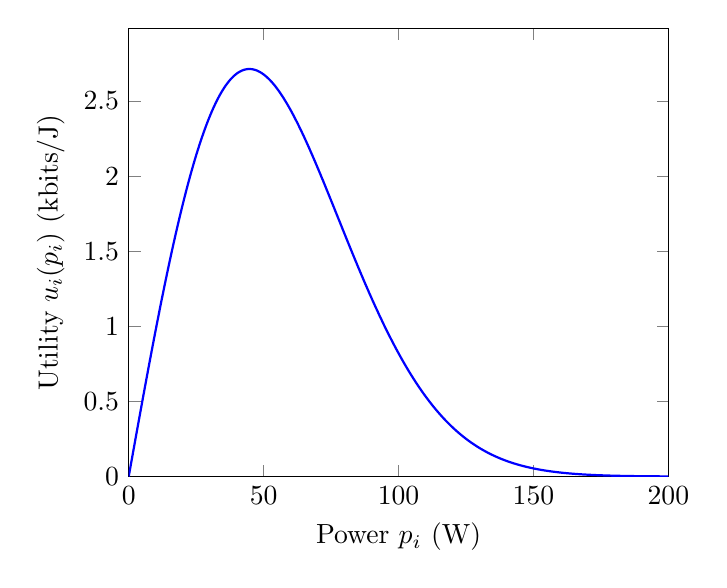
\begin{tikzpicture}
            \begin{axis}[
                    ylabel = {Utility $u_i(p_i)$ (kbits/J)},
                    xlabel = {Power $p_i$ (W)},
                    domain = 0:200,
                    samples = 1000,
                    xmin = 0,
                    xmax = 200,
                    ymin = 0
                ]
                \addplot[
                    color = blue,
                    thick
                ]
                {(x/10)*exp(-x^2/(2*2000))};
            \end{axis}
        \end{tikzpicture}
        \caption{Example of an utility function for a player}
    \end{figure}
\end{frame}

\note{
    Intuition behind this utility function:
    \begin{itemize}
        \item If $p_i$ is too low, the signal from player $i$ suffers too much from interference
        and is not well received by the base station.
        \item If $p_i$ is too high, the battery level of player $i$ is decreasing too quickly.
    \end{itemize}
}

\begin{frame}{The single-shot game}
    \begin{block}{Where is the game here?}
        Increasing $\text{SINR}_i$ requires increasing $p_i$, this will decrease $\text{SINR}_j$ and
        thus decrease other players utility.
    \end{block}
    \pause 
    \vspace{0.5cm}
    \begin{alertblock}{The Nash Equilibrium of the single-shot game is Pareto inefficient}
        In the same way the Nash Equilibrium of the single-shot Prisoner's Dilemma is
        Pareto inefficient...
    \end{alertblock}
    \pause
    \vspace{0.5cm}
    \textbf{{\color{green}Can we do better in a repeated game settings to force a better outcome?}}
\end{frame}

\begin{frame}{The repeated game model}
    \begin{exampleblock}{The repeated game model}
        \begin{itemize}
            \pause
            \item \textbf{Rounds}: a round corresponds to a packet transmission.
            \pause
            \item \textbf{Criterion for ranking payoffs}: we use the $\delta$-discounted average with a
            discount factor $\delta$ very close to 1 (can you guess why?).
            \pause
            \item \textbf{Signals}: after each transmitted packet, the base station informs each player
            of the received power level of each user.
            \pause
            \item \textbf{State of nature}: two possible cases
            \begin{enumerate}
                \pause
                \item the power attenuations $h_i$ are constant: only one state\\
                $\to$ standard repeated game,
                \pause
                \item the power attenuations $h_i$ vary in time: multiple states\\
                $\to$ stochastic game.
            \end{enumerate}
        \end{itemize}
    \end{exampleblock}
\end{frame}

\note{
    $\delta$ is very close to 1 because the time slot for the transmission of a single packet
    is typically very short (on the order of a few tens of microseconds).
}

\begin{frame}{Equilibrium strategy}
    \begin{block}{Equilibrium strategy}
        \begin{itemize}
            \item As long as no users exceeds the received power level, the system operates normally ;
            \item If a player behaves selfishly, all the other players transmit at maximum power level
            during the next time slot as a punishment.
        \end{itemize}
    \end{block}

    \vspace{0.5cm}
    \textbf{{\color{green}This strategy forms a new equilibrium more Pareto efficient than the
    single-shot Nash equilibrium.}}
\end{frame}
